\section{Background}
In this chapter we will give some background knowledge about the technologies we will be working with: The service oriented programming language Jolie and the wire-level Advanced Message Queue Protocol.
\subsection{Service-oriented architectures}
As mention before Jolie is a service oriented programming language, but what does that mean exactly?\\
Service oriented programs does not expose an interface of methods but an interface of service-calls. Each service invoke other services methods through standardized communication protocols. Service-oriented architectures are easy to modularize and they are very scalable. The easy modularization and scalability of service-oriented architectures makes them ideal for distributed systems.
\subsection{Jolie}
Jolie\footnote{\url{http://www.jolie-lang.org}} is an interpreted language running on the Java Virtual Machine. Jolie makes it extremely easy to host a web service and invoke others.\\
Jolie supports a growing number of protocols and Jolie promise to keep behavior and deployment separated. What this means is that the code one writes does not need to be changed when one changes the protocol. One simply choose another Jolie supported protocol and the program functions as always. This will prove a challenge for us in extending the language while still keeping the promise of behavior and deployment separation.
\subsection{Advanced Message Queuing Protocol}
Message queues are being more and more used in event-based and message-oriented software architectures. They are also ideal for handling large amounts of data because you can simply queue something for processing and handle the flow of data as quickly as you can. AMQP\footnote{\url{http://www.amqp.org}} is an open standard application layer protocol for message-oriented middleware.\\
AMQP's defining features include message orientation, queuing, routing, security and reliability.
\subsubsection{Queues and Exchanges explained}
A \textit{Publisher} publishes messages to an \textit{Exchange}.\\
An exchange is defined with an exchange type (routing algorithm). AMQP 0.9.1 describes support for four types\footnote{\url{https://www.rabbitmq.com/amqp-0-9-1-reference.html}}:
\begin{itemize}
\item Direct
\item Fanout
\item Topic
\item Headers/Match
\end{itemize}
A \textit{Queue} may bind to one or more exchanges and thereby receive messages to hold. A queue may bind with a routing key to only receive messages with matching routing criteria.\\
A message handler is called a \textit{Consumer}. A consumer consumes messages by subscribing to a single queue.
\begin{figure}[H]
  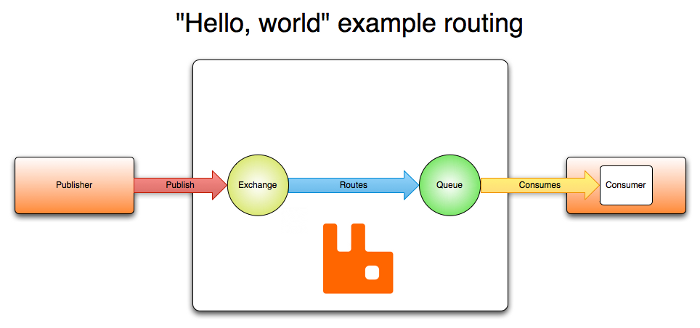
\includegraphics[width=\textwidth]{illustrations/publisher-exchange-queue-consumer.png}
  \caption{AMQP message path\footnote{\url{https://www.rabbitmq.com/tutorials/amqp-concepts.html}}}
\end{figure}
\newpage